\documentclass[a4paper,12pt]{article}
\usepackage[T2A]{fontenc}
\usepackage[utf8x]{inputenc}
\usepackage[english,russian]{babel}
\usepackage{amssymb,amsfonts,amsmath,mathtext}
\usepackage[unicode]{hyperref}
\usepackage{listings}
\usepackage{graphicx}
\usepackage{float}
\graphicspath{{images/}}
\newcommand{\anonsection}[1]{\section*{#1}\addcontentsline{toc}{section}{#1}}

\begin{document}

% Титульный лист

\begin{titlepage}
\newpage

\begin{center}

\textit{Министерство науки и высшего образования Российской Федерации \\ 
Федеральное государственное бюджетное образовательное \\
учреждение высшего образования \\
«Московский государственный технический университет \\
имени Н.Э. Баумана (национальный исследовательский университет)» \\
(МГТУ им. Н.Э. Баумана) \\}
\hrulefill
\end{center}

\vspace{2em}

\begin{flushleft}
ФАКУЛЬТЕТ <<Информатика и системы управления>> \\
\vspace{0.5em}
КАФЕДРА <<Программное обеспечение ЭВМ и информационные технологии>>
\end{flushleft}


\vspace{8em}

\begin{center}
\LARGE Лабораторная работа №5 \\
\end{center}

\vspace{1.5em}

\begin{center}
\textsc{Конвейер}
\end{center}

\vspace{6em}

\begin{center}
Головнев Н.В.

\vspace{4em}

ИУ7-54Б
\end{center}

\vspace{\fill}

\begin{center}
Москва 2019
\end{center}

\end{titlepage}

\tableofcontents

% Введение

\newpage
\anonsection{ВВЕДЕНИЕ}
Конвейер — машина непрерывного транспорта, предназначенная для перемещения сыпучих, кусковых или штучных грузов. Важной характеристикой работы конвейера является её непрерывность. Это верно и когда конвейером называют средство для транспортировки грузов на небольшие расстояния, и когда конвейер — система поточного производства на базе двигающегося объекта для сборки. Эта система превратила процесс сборки сложных изделий, ранее требовавший высокой квалификации от сборщика, в рутинный, монотонный, низкоквалифицированный труд, значительно повысив его производительность. Расстановка рабочих или автоматов на линии конвейерной сборки осуществляется с учётом технологии и последовательности сборки или обработки деталей, чтобы добиться эффективного разделения труда.
На основе принципа работы конвейера была придумана модификация процессоров (например, процессоры от Intel архитектуры P6).
Конвейерное производство можно также рассматривать как отдельный паттерн проектирования программных систем.

\newpage
\anonsection{ПОСТАНОВКА ЗАДАЧИ}
Цель задачи: Изучить и разработать алгоритм конвеерной обработки, используя многопоточность.
Задача: написать приложение для создания и генерирования параметров автомобиля и вывести данные об автомобилях в отдельный файл. Параметры создаются и распределяются между автомобилями по случайному закону.

\newpage
\section{АНАЛИТИЧЕСКАЯ ЧАСТЬ}
\subsection{Описание алгоритмов}
Многие системы требуют эффективно и компактно реализовать механизм обработки потока событий/запросов/сообщений в системах с потенциально большим количеством обработчиков. В таких случаях, в качестве главного шаблона проекта берут шаблон "Цепочка обязанностей".
Идея шаблона заключается в организации рекуррентного конвейера из обработчиков, в котором каждый обработчик может либо обработать поступившее сообщение (например, только сообщения определенного типа), либо делегировать обработку следующему в конвейере обработчику. Возможен еще вариант обработки и последующей передачи. При этом, клиенту, чтобы инициировать обработку того или иного сообщения достаточно лишь передать его первому в конвейере обработчику[\ref{link:link1}].
Зачастую, бывает ситуация, когда обработка сообщений требует высокоскоростных вычислений, большая часть обработчиков "простаивает" в ожидании результата работы одного, какого-то обработчика, который владеет ресурсом в данный момент.
В данном случае, работу каждого обработчика осуществляют через отдельный поток, который, в результате своей работы отправляет обработанное сообщение в очередь работы следующего обработчика, после этого сразу же обрабатывая следующее поступившее сообщение. Данная многопоточная система значительно ускоряет обработку сообщений, в отличие от однопоточного варианта.
\begin{figure}[h]
\center{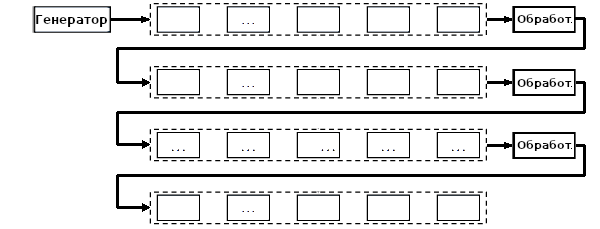
\includegraphics[scale=0.75]{conveyer.png}}
\caption{Пример конвейера}
\label{images:example1}
\end{figure}
Однако, в результате работы такой системы, может возникнуть ситуация, когда потоки одновременно работают с одной и той же критической секцией (один поток записывает в очередь, другой из нее читает), вследствие чего может возникнуть неопределенное поведение(undefined behaviour) или даже ошибка доступа(SEGFAULT, double free и тд...). Для того, чтобы такие ситуации не возникали, используются специальные механизмы синхронизации, которые используют мьютексы, семафоры и условные переменные.

\newpage
\subsection{Вывод}
В данном разделе были описаны способы решения поставленной задачи - реализовать конвейер по <<производству автомобилей>> со случайными параметрами. Конвейерный метод обработки прост - необходимо провести каждый элемент (<<автомобиль>>) через каждый обработчик и в конце вывести в файл (конечный обработчик). В случае распараллелирования задачи, каждый обработчик работает как отдельный поток, который берет из очереди отдельное сообщение, обрабатывает и кладет в очередь следующего обработчика, который также работает в отдельном потоке.

\newpage
\section{КОНСТРУКТОРСКАЯ ЧАСТЬ}
\subsection{Разработка алгоритмов}
Каждый поток обладает счетчиком, которому присваивается значение, равное количеству элементов в изначально сгенерированном массиве объектов. 
Каждый поток должен работать следующим образом:
\begin{enumerate}
\item Извлекать данные из предыдущей очереди, синхронизируя процесс получения данных с предыдущим потоком, чтобы не возникало состояния "гонок", если данных в предыдущей очереди нет, то ждать, пока данные в ней не будут доступны;
\item Обработать данные;
\item Декрементировать значение счетчика;
\item Передать данные в следующую очередь, синхронизация процесс передачи со следующим потоком, чтобы не возникало состояния "гонок";
\item Если счетчик потока не обнулился, то продолжить работу, иначе завершить.
\end{enumerate}

Обработка данных осуществляется в отдельной функции. Все используемые функции должны иметь одинаковый интерфейс. Это нужно вследствие удобства разработки системы и ее последующей модификации в случае надобности.
В качестве параметра этой функции передается обрабатываемый объект (или ссылка на него).

\newpage
\subsection{Вывод}
На основе данных, изложенных в аналитической части, были разработаны окончательные требования к разрабатываемым алгоритмам. Теперь можно преступить непосредственно к созданию требований к программному обеспечению и разработке алгоритмов.

\newpage
\section{ТЕХНОЛОГИЧЕСКАЯ ЧАСТЬ}
\subsection{Требования к программному обеспечению}
Программа должна работать на операционной системе Arch Linux. Количество создаваемых автомобилей заранее известно и заложено в программе. Результат работы должен записываться в файл result.txt. Данные должны выводиться в виде описания автомобиля. Например: номер - 111, цвет - жёлтый и тд...

\newpage
\subsection{Средства реализации}
Для реализации данных алгоритмов был выбран язык программирования С, компилятор gcc и некоторые функции из библиотеки glibc (memcpy, malloc и тд...). \\
Основные особенности Си:
\begin{itemize}
\item простая языковая база, из которой в стандартную библиотеку вынесены многие существенные возможности, вроде математических функций или функций работы с файлами;
\item ориентация на процедурное программирование;
\item использование препроцессора для абстрагирования однотипных операций;
\item доступ к памяти через использование указателей;
\item передача параметров в функцию по значению, а не по ссылке (передача по ссылке эмулируется с помощью указателей);
\item наличие указателей на функции и статических переменных;
\item области видимости имён;
\item структуры и объединения — определяемые пользователем собирательные типы данных, которыми можно манипулировать как одним целым.
\end{itemize}

\newpage
\subsection{Листинг кода}
\lstdefinestyle{customc}{
  belowcaptionskip=1\baselineskip,
  breaklines=true,
  frame=L,
  xleftmargin=\parindent,
  language=C,
  showstringspaces=false,
  basicstyle=\footnotesize\ttfamily
}
В листингах (\ref{listings:listing1})(\ref{listings:listing2})(\ref{listings:listing3}) представлены реализации поточных функций, осуществляющих взаимодействие с "конвейерной лентой" и обрабатывющих объекты используемой функцией.
\lstinputlisting[captionpos=b, caption=\label{listings:listing1}Реализация функции первого потока, style=customc]{listing1.c}
\newpage
\lstinputlisting[captionpos=b, caption=\label{listings:listing2}Реализация функции любого потока\, кроме первого и последнего, style=customc]{listing2.c}
\newpage
\lstinputlisting[captionpos=b, caption=\label{listings:listing3}Реализация функции последнего потока, style=customc]{listing3.c}

\newpage
\subsection{Вывод}
Используя язык программирования C, в ходе практической работы была спроектирована и написана реализация алгоритма конвейерной обработки с использованием многопоточности.

\newpage
\section{ЭКСПЕРИМЕНТАЛЬНАЯ ЧАСТЬ}
\subsection{Характеристики аппаратного и программного обеспечения}
% Часть которую никогда нельзя менять
Тестирование приложения проводилось на машине со следующими характеристиками:\\
\begin{itemize}
\item Процессор Intel® Core™ i7-7700HQ;
\item Оперативная память 16 ГБ;
\item Операционная система - Arch Linux с рабочим окружением Cinnamon.
\end{itemize}

\newpage
\subsection{Примеры работы}
На рис. \ref{images:example1} демонстрируется работа приложения. Запуск приложения осуществляется из эмулятора терминала в Arch Linux. Также на рис. \ref{images:example2} показан результат работы приложения, выведенный в файл. 
\begin{figure}[h]
\center{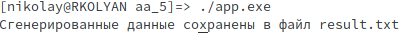
\includegraphics[scale=1]{example1.png}}
\caption{Пример работы приложения}
\label{images:example1}
\end{figure}
\begin{figure}[H]
\center{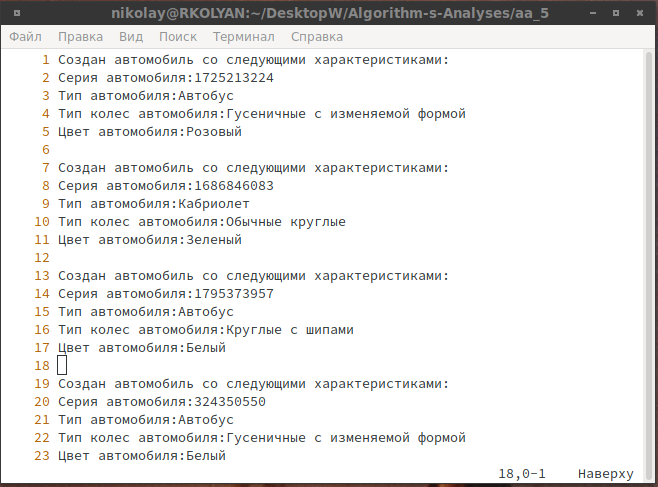
\includegraphics[scale=0.65]{example2.png}}
\caption{Результат приложения, выведенный в файл}
\label{images:example2}
\end{figure}

\newpage
\subsection{Вывод}
В данном разделе была показана работа программы, разработанной согласно требованиям из конструкторской и технологической части. Пример запуска программы 
был показан в Arch Linux. Результатом программы стало множество выведенных в отдельный файл сообщений с данными, сгенерированными в результате работы приложения.

\newpage
\anonsection{ЗАКЛЮЧЕНИЕ}
В данной лабораторной работе была спроектирована и реализована многопоточная программа, реализующая конвейерную обработку объектов. Данная реализация была написана на Си с использованием функций для работы с потоками, взятые из стандартной библиотеки (заголовочный файл - threads.h). Каждый отдельный поток выполняет функцию отдельной "ленты" конвейера, в которой объекты извлекаются из предыдущей очереди, обрабатываются и сохраняется в следующей очереди (очереди в следующей "ленте"). Работа потоков прекращается, если счетчик объектов обнуляется. Результат работы приложения сохранаяется в отдельный файл result.txt, на этом результат работы приложения заканчивается.
Преимущество такого подхода обработки данных по сравнению с линейным является то, что в момент времени, пока один объект обрабатывается во одном потоке, в другом происходит обработка другого, таким образом весь конвейер не проставивает только из-за обработки одного объекта. В линейном же случае, каждый отдельный объект проходит весь конвейер, другие же объекты не могут быть обработаны.
Многопоточные версии таких алгоритмов могут применяться для обработки большого количества объектов, где обрабатываемые объекты нужно обработать немедленно.

\newpage
\anonsection{СПИСОК ИСТОЧНИКОВ}
\begin{enumerate}
\item Хабр, паттерн проектирования "Цепочка обязанностей" - \url(https://habr.com/ru/post/113995/)\label{links:link1}
\item 
\end{enumerate}

\end{document}
